\documentclass[addpoints,11pt]{exam}

\usepackage{alltt}
\usepackage[margin=1in]{geometry}   % set up margins
\usepackage[T1]{fontenc}
\usepackage[usenames,dvipsnames]{xcolor}
\usepackage{enumerate}              % fancy enumerate
\usepackage{amsmath}                % used for \eqref{} in this document
\usepackage{amsthm}
\theoremstyle{definition}
\newtheorem{exmp}{Example}[section]
\usepackage{verbatim}               % useful for \begin{comment} and \end{comment}
\usepackage{eurosym}                % used for euro symbol
\usepackage{caption} 
\usepackage{graphicx}
\graphicspath{{Figures/}}
\usepackage{subcaption}
\usepackage{color}
\usepackage{float}
\usepackage{amssymb}
\usepackage{sgamevar}
\usepackage{sgame}
\usepackage[colorlinks=true]{hyperref}
\hypersetup{colorlinks=true, citecolor=ForestGreen, linkcolor=BlueViolet, urlcolor=Magenta}



%Solutions or nah (blank next two lines out for no solutions, unblank #3)
%\printanswers
%\newcommand{\dd}[1]{\par {\textbf{\textcolor{red}{#1}}}}
\newcommand{\dd}[1]{}  


\setlength\parindent{0pt}
\unframedsolutions
\SolutionEmphasis{\color{red}}
\CorrectChoiceEmphasis{\color{red}}
\renewcommand{\choicelabel}{(\alph{choice})}
\newcommand{\blank}[0]{\underline{\hspace{3cm}}}
\pointformat{\bfseries[\thepoints]}
\pointpoints{pt}{pts}
\pointsinrightmargin

\begin{document}
	
\title{\textbf{Final Exam} \\ \dd{Solutions\\} \vspace{2 mm} {\large ECON 101}}
\author{Summer I 2015}
\date{}
\maketitle

\makebox[\textwidth]{Name:\enspace\hrulefill}
\\

\makebox[\textwidth]{ONYEN:\enspace\hrulefill}
\\

\makebox[\textwidth]{PID:\enspace\hrulefill}
\\

\makebox[\textwidth]{Honor Code Signature:\enspace\hrulefill}
	
\begin{center}
	\fbox{\fbox{\parbox{5.5in}{\centering
			This exam consists of 50 multiple choice questions and 2 short answer questions. Multiple choice questions should be bubbled in on a scantron. Extra paper for scratch work is attached. The total number of points available on this exam is \textbf{100}.}}}
\end{center}

\section*{Multiple Choice [1.5 pts each]}

Choose the option that best answers the question given.

\begin{questions}
	
\question Suppose a per unit tax of \$.50 is imposed on buyers of Pepsi. As a result, the price buyers end up paying is \$1.25 for each can. Moreover, the amount Pepsi-Cola receives for every can of Pepsi sold decreases by \$.15. Given this, we can say that \underline{\hspace{3cm}} bore most of the tax burden and the equilibrium price of Pepsi before the tax was imposed was \underline{\hspace{3cm}}.


\begin{choices}
	\choice sellers; \$.75
	\CorrectChoice buyers; \$.90
	\choice sellers; \$.90
	\choice buyers; \$.75
\end{choices}


\question Firms in monopolistically competitive markets are similar to monopolies in that they both \underline{\hspace{3cm}} and are similar to firms in perfectly competitive markets in that they both \blank.

\begin{choices}
	\choice make positive profits in the short and long run; are price takers
	\choice charge a price above the marginal cost; produce at the efficient scale in the long run
	\CorrectChoice are price makers; make zero economic profit in the long run
	\choice are in markets with barriers to entry; produce at the efficient quantity
\end{choices}

\newpage

\question Suppose the supply curve of neck ties shifts such that the market price for neck ties decreases. Which of the following statements must be true?

	\begin{enumerate}[i.]
		\item Producer surplus decreases due to the lower price of neck ties.
		\item Consumer surplus increases as existing buyers in the market pay lower prices on the neck ties they were already willing to buy.
		\item New buyers enter the market as a result of the price decrease and realize surplus.
	\end{enumerate}

\begin{choices}
		\choice i and iii
		\choice i and ii
		\CorrectChoice ii and iii
		\choice i, ii, and iii
\end{choices}

\uplevel{For questions \ref{q4}-\ref{q5}, refer to Figure \ref{MC1} below, which shows demand curves relating to some good $A$.}

\begin{figure}[H]
	\centering
	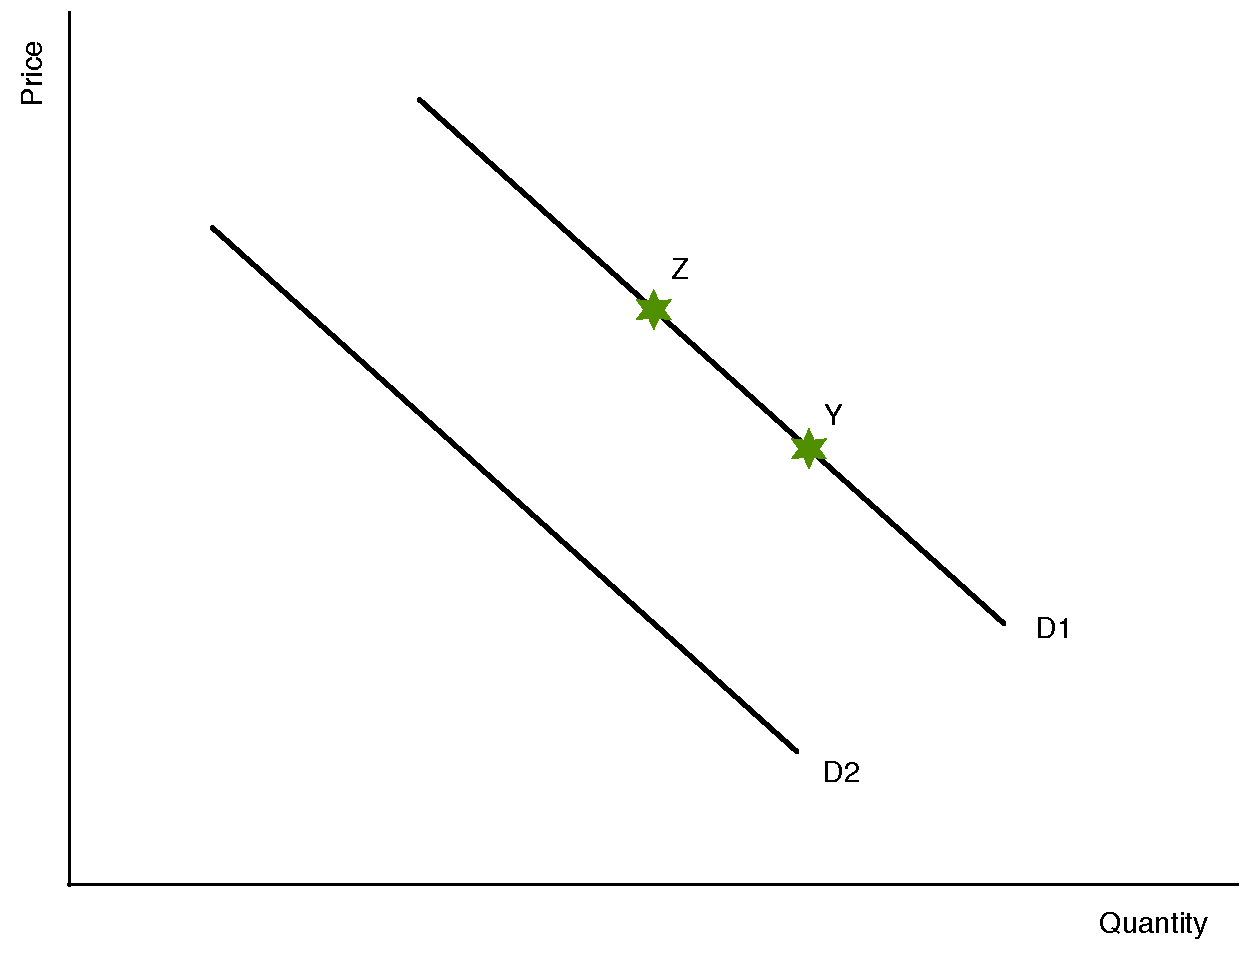
\includegraphics[scale=.38]{Exam1_MC2.pdf}
	\caption{Demand for Good $A$}
	\label{MC1}
\end{figure}

\question \label{q4} Suppose the cross-price elasticity between goods $A$ and $B$ is $-2.5$. All else equal, a decrease in the price of good $B$ would cause a move from  

\begin{choices}
	\CorrectChoice D2 to D1.
	\choice Y to Z.
	\choice Z to Y.
	\choice D1 to D2.
\end{choices}


\question \label{q5} All else equal, an increase in the price of good $A$ would cause a move from

\begin{choices}
	\choice D2 to D1.
	\CorrectChoice Y to Z.
	\choice Z to Y.
	\choice D1 to D2.
\end{choices}

\newpage

\question Suppose the CPI in 1990 using 1980 as the base year was 114, while the CPI in 1980 using 1975 as the base year was 105. If average salary of engineers in 1990 was \$74,500 and they were equally as well off in terms of purchasing power as engineers were in 1980, then the average salary of engineers in 1980 must have been approximately

\begin{choices}
	\CorrectChoice \$65,351.
	\choice \$84,930.
	\choice \$74,500.
	\choice \$68,618.
\end{choices}

\question Refer to Figure \ref{MC5}. 

\begin{figure}[H]
	\centering
	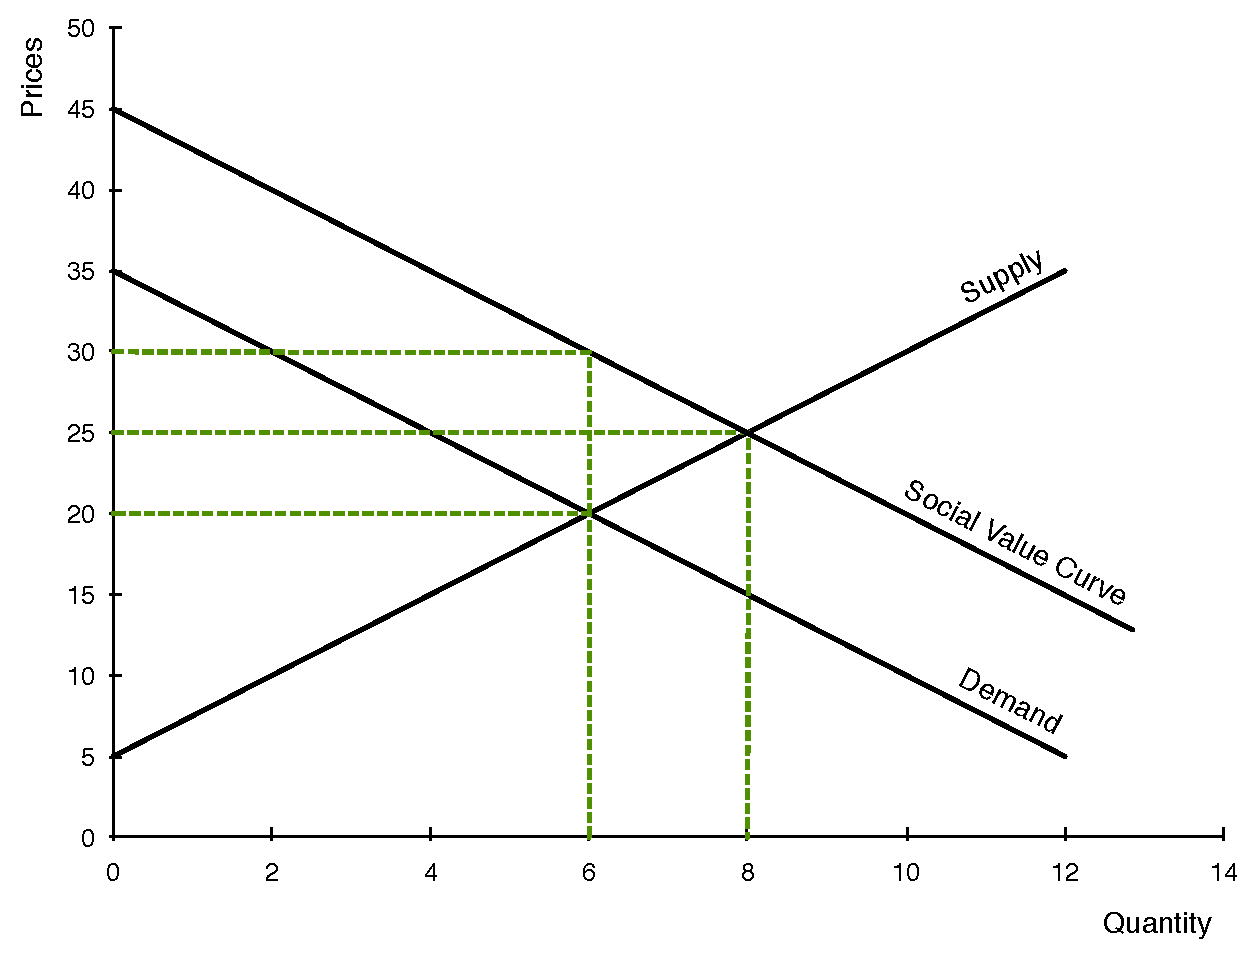
\includegraphics[scale=.40]{Exam_Review5.pdf}
	\caption{A Market Externality}
	\label{MC5}
\end{figure}

If the quantity exchanged in the market increased from the 6 units to 8 units, then the total external benefit realized would increase by \underline{\hspace{3cm}}, while deadweight losses would decrease by \blank.

\begin{choices}
	\choice \$20; \$20
	\choice \$10; \$20
	\choice \$10; \$10
	\CorrectChoice \$20; \$10
\end{choices}

\question For a firm in a monopolistically competitive market, which of the following accurately describes the relationship between the price, average total cost, and marginal cost in the short run given that the firm is making a negative profit?

\begin{choices}
	\choice $ATC = P = MC$
	\choice $ATC > P = MC$
	\choice $ATC = P > MC$
	\CorrectChoice $ATC > P > MC$
\end{choices}

\newpage

\question Consider Figure \ref{MC8}, which shows the market for money in Portlandia. $P$ is the overall price level in the economy.

\begin{figure}[H]
	\centering
	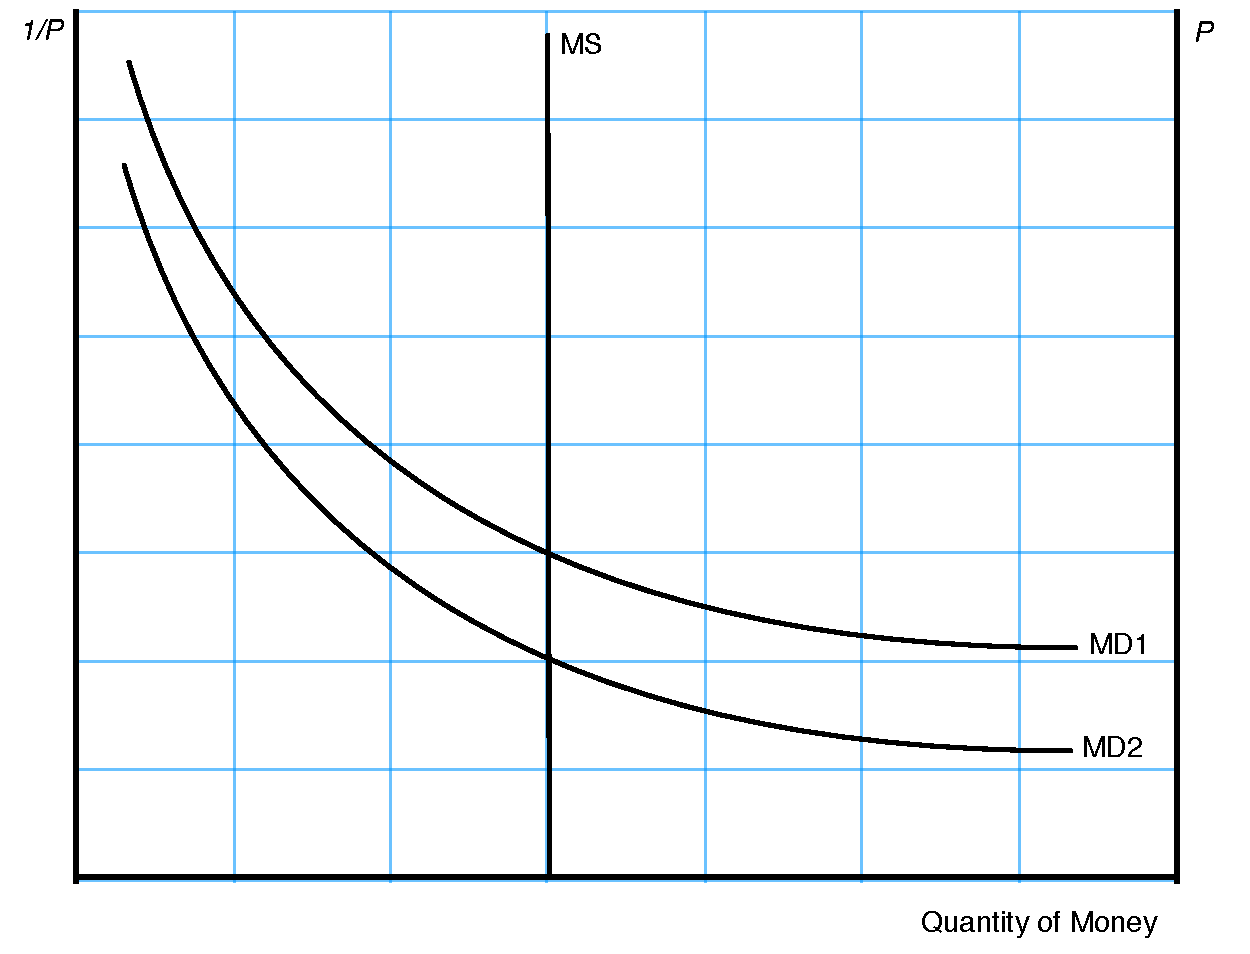
\includegraphics[scale=.40]{Final_MC8.pdf}
	\caption{The Money Market}
	\label{MC8}
\end{figure}

If the demand for money shifts from MD1 to MD2, then we can say that 

\begin{choices}
	\choice the value of money will increase, while the price level will decrease.
	\choice the value of money and the price level will both increase.
	\CorrectChoice the value of money will decrease, while the price level will increase.
	\choice the value of money and the price level will both decrease.
\end{choices}

\question Keystone Fireworks has fixed costs of \$10 and the marginal costs outlined in Table \ref{MC9}.

\begin{table}[ht]
	\caption{Marginal Costs for Cheerwine}
	\label{MC9}
	\centering
	\begin{tabular}{  c| c}   
		Quantity & Marginal Cost\\
		\hline
		1 & \$2 \\
		2 & \$4 \\
		3 & \$7 \\
		4 & \$11 \\
		5 & \$16 \\
		6 & \$22 \\
	\end{tabular}
\end{table}

What is the average total cost of producing the fifth unit?

\begin{choices}
	\choice \$3.20
	\CorrectChoice \$10.00
	\choice \$5.20
	\choice \$8.00
\end{choices}

\newpage


\question Consider Table \ref{MC10}, which shows the environment faced by a monopolist.


\begin{table}[ht]
	\caption{Market Environment}
	\label{MC10}
	\centering
	\begin{tabular}{  c| c | c }   
		Output & Total Revenue &  Variable Costs \\     
		\hline
		1 & \$50 & \$30 \\
		2 & \$80 & \$60 \\
		3 & \$90 & \$90 \\
		4 & \$80 & \$120  \\
		5 & \$50& \$150 \\
		6 & \$20& \$180 \\
		7 & \$10 & \$210 \\
	\end{tabular}
\end{table}

What price will this firm charge in order to maximize profits?

\begin{choices}
	\CorrectChoice \$40
	\choice \$30
	\choice \$20
	\choice \$10
\end{choices}


\question Consider the simultaneous move game between Righty and Lefty shown below, where the first number in each block is the payoff to Lefty and the second is the payoff to Righty.

\renewcommand{\gamestretch}{1.5}
\sgcolsep=25pt
\begin{figure}[htb]\hspace*{\fill}%
	\begin{game}{2}{2}[Lefty][Righty] 
		&  Swerve & Straight \\
		Swerve & 2, 2 & $x$, 4 \\
		Straight & 1, $y$ & 2, 3 \\
	\end{game} 
	\hspace*{\fill}%
\end{figure}

If this particular game has \textit{no} Nash equilibrium, then possible values of $x$ and $y$ are

\begin{choices}
	\choice $x=1$ and $y=2$.
	\CorrectChoice $x=1$ and $y=4$.
	\choice $x=3$ and $y=2$.
	\choice $x=3$ and $y=4$.
\end{choices}

\question Suppose you currently hold a bond that promises to pay \$100 in a year, \$100 in two years, and \$1,100 in three years. If you wish to sell the bond today in order to buy a new bicycle, which of the following market interest rates would allow you to sell the bond for the highest price?
\begin{choices}
	\choice 7\%
	\choice 10\%
	\CorrectChoice 5\%
	\choice 8\%
\end{choices}



\uplevel{For questions \ref{q14}-\ref{q15}, refer to Figure \ref{MC14}. Suppose an economy is operating at point $G$ and assume this position came about through a permanent demand side shock.}


	\begin{figure}[H]
		\centering
		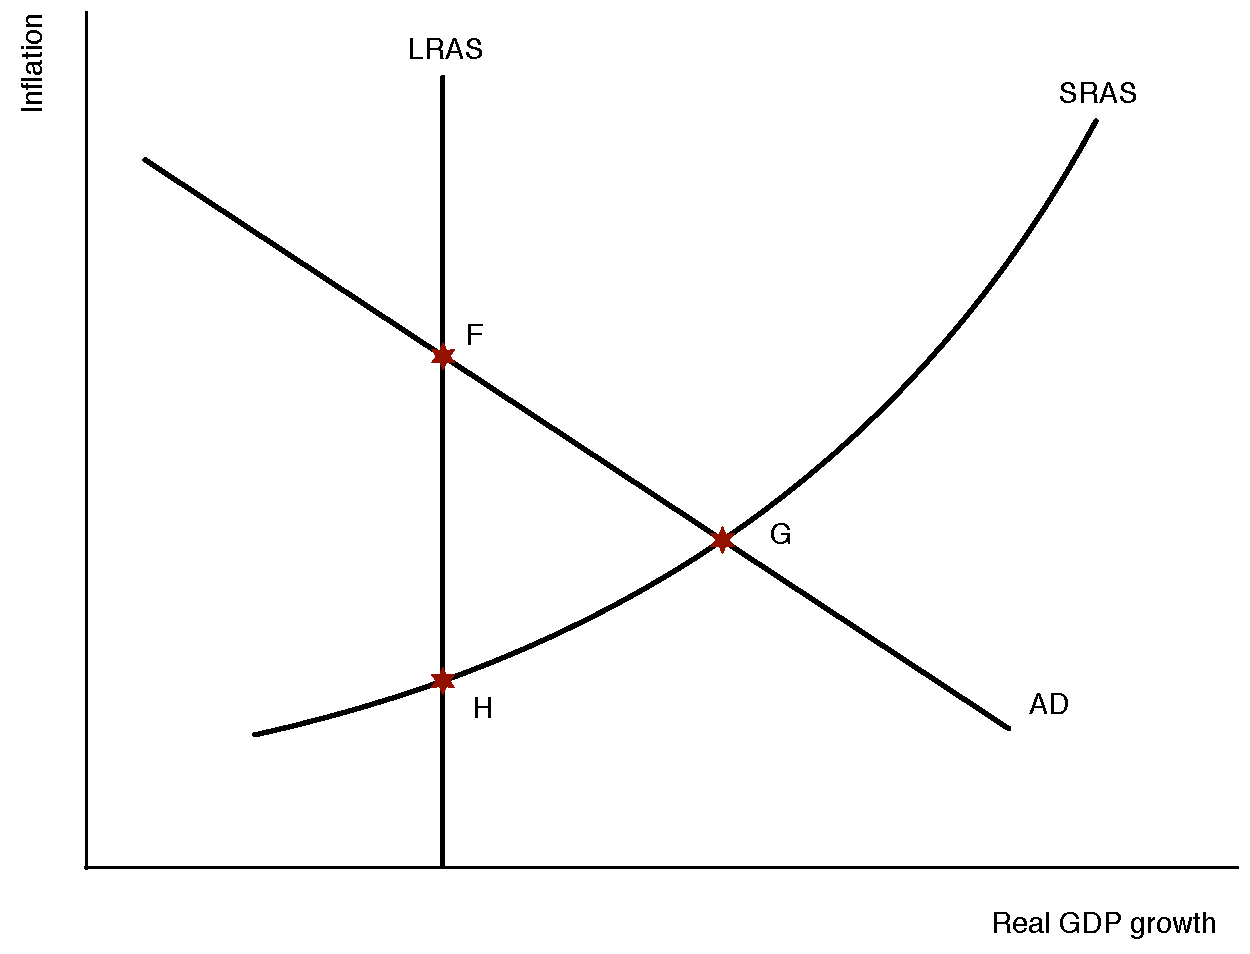
\includegraphics[scale=.38]{Final_MC14.pdf}
		\caption{AS-AD Model}
		\label{MC14}
	\end{figure}
	
	\question \label{q14} At point $G$, actual inflation is \blank than expected inflation, and real GDP growth is \blank the natural rate.
	
	\begin{choices}
		\choice less; above 
		\choice less; below
		\choice greater; below
		\CorrectChoice greater; above
	\end{choices}
	
	\question \label{q15} In the absence of monetary or fiscal policy, as the economy transitions to its long-run equilibrium,
	
	\begin{choices}
		\choice expected inflation will increase and real GDP growth will increase.
		\choice expected inflation will decrease and real GDP growth will increase.
		\CorrectChoice expected inflation will increase and real GDP growth will decrease.
		\choice expected inflation will decrease and real GDP growth will decrease.
	\end{choices}
	
	\question A market is currently at equilibrium. A price floor above the equilibrium price is imposed, leading to \blank in consumer surplus and \blank in total surplus.
	
	\begin{choices}
		\choice a decrease; an increase
		\choice an increase; an increase
		\CorrectChoice a decrease; a decrease
		\choice no change; no change
	\end{choices}

	
	\question Which of the following is NOT a cost of inflation?
	
	\begin{choices}
		\choice Shoeleather costs
		\CorrectChoice Relative-price stability
		\choice Arbitrary redistribution of wealth
		\choice Menu costs
	\end{choices}
	


\uplevel{For questions \ref{q18} - \ref{q19}, refer to Figure \ref{MC18}, which shows the production possibilities of two brothers, Jony and Dany.}


\begin{figure}[H]
	\centering
	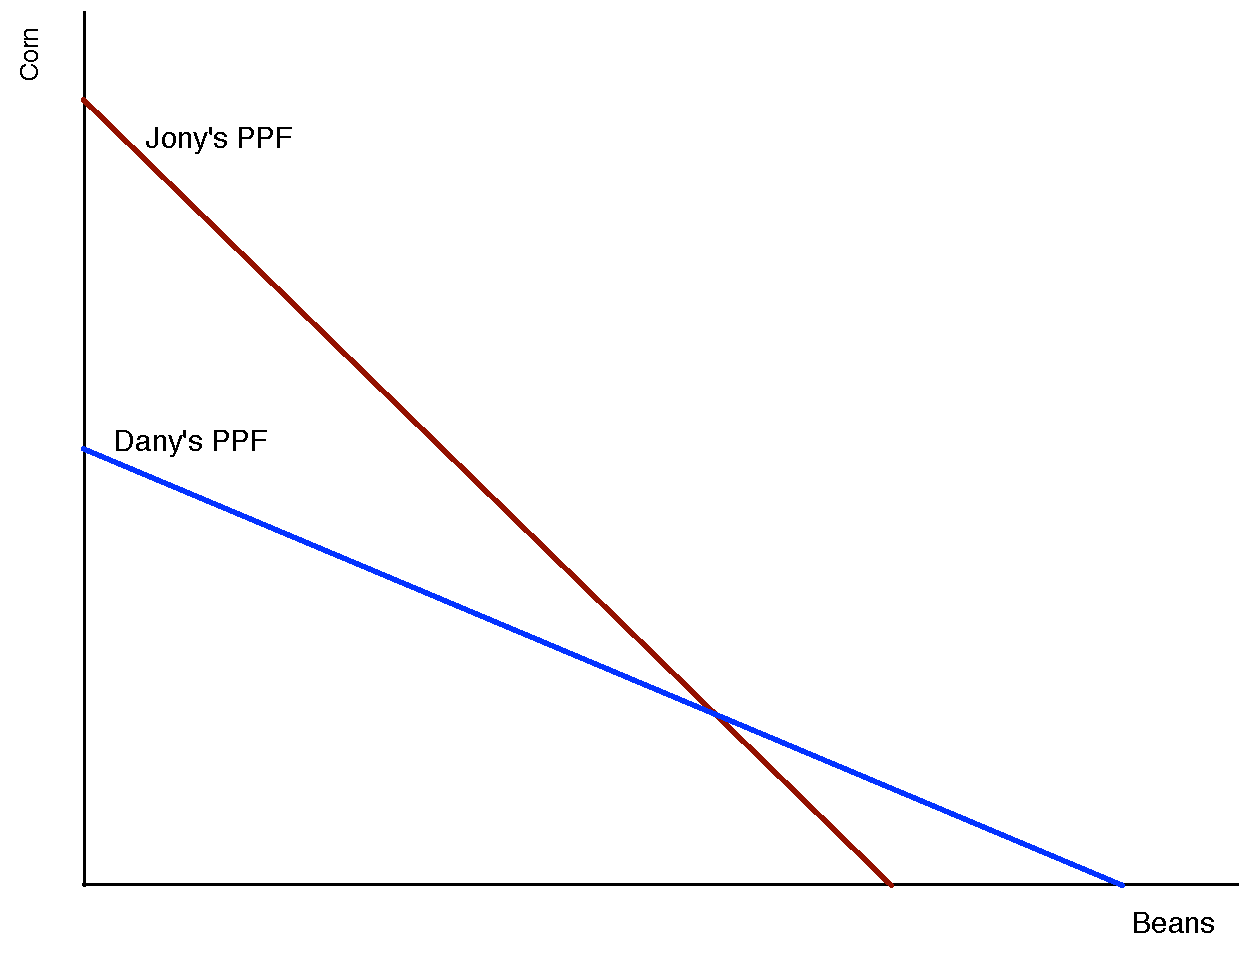
\includegraphics[scale=.4]{Final_MC18.pdf}
	\caption{Production of Beans and Corn}
	\label{MC18}
\end{figure}

	
	\question \label{q18} From their respective PPFs, we can conclude that
	
	\begin{choices}
		\CorrectChoice Dany has an absolute advantage in the production of beans, while Jony has an absolute advantage in the production of corn.
		\choice Dany has an absolute advantage in the production of both beans and corn.
		\choice Dany has an absolute advantage in the production of corn, while Jony has an absolute advantage in the production of beans.
		\choice Jony has an absolute advantage in the production of both beans and corn.
	\end{choices}
	
	\question \label{q19} Additionally, we can also say that 
	
	\begin{choices}
		\choice Jony has a comparative advantage in both goods, and Dany has a comparative advantage in neither good.
		\choice Jony has a comparative advantage in neither good, and Dany has a comparative advantage in both goods.
		\CorrectChoice Jony has a comparative advantage in corn, and Dany has a comparative advantage in beans.
		\choice Jony has a comparative advantage in beans, and Dany has a comparative advantage in corn.
		\choice None of the above. Not enough information given.
	\end{choices}
	
\newpage
	
	\question Jack and Jill are the only lemonade providers in Jurassic World. They face the environment outlined in Table \ref{MC21}. 
	
	\begin{table}[H]
		\caption{Demand Schedule and Costs Lemonade}
		\centering
		\begin{tabular}{c|c|c}
			Price & Quantity Demanded & Average Total Cost \\
			\hline
			\$1.00 & 400 & \$.30\\
			\$.90 & 500 & \$.30\\
			\$.80 & 600 & \$.30 \\
			\$.70 & 700 & \$.30 \\
			\$.60 & 800 & \$.30 \\
		\end{tabular} 
		\label{MC21}
	\end{table}
	
	The two friends currently have an agreement where they produce 600 drinks in total and split production evenly. If Jack were to break this agreement and increased his lemonade stand's production by 100 drinks while Jill stuck to the original agreement, the profit realized by Jack would now be \blank and the profit realized by Jill would be \blank.
	
	\begin{choices}
		\CorrectChoice \$160; \$120
		\choice \$140; \$140
		\choice \$160; \$140
		\choice \$280; \$210
	\end{choices}
	
	
	\question Figure \ref{MC22} shows the production function of a small country, as well as its investment and depreciation functions. Assume there is no population growth.
	
	
	\begin{figure}[H]
		\centering
		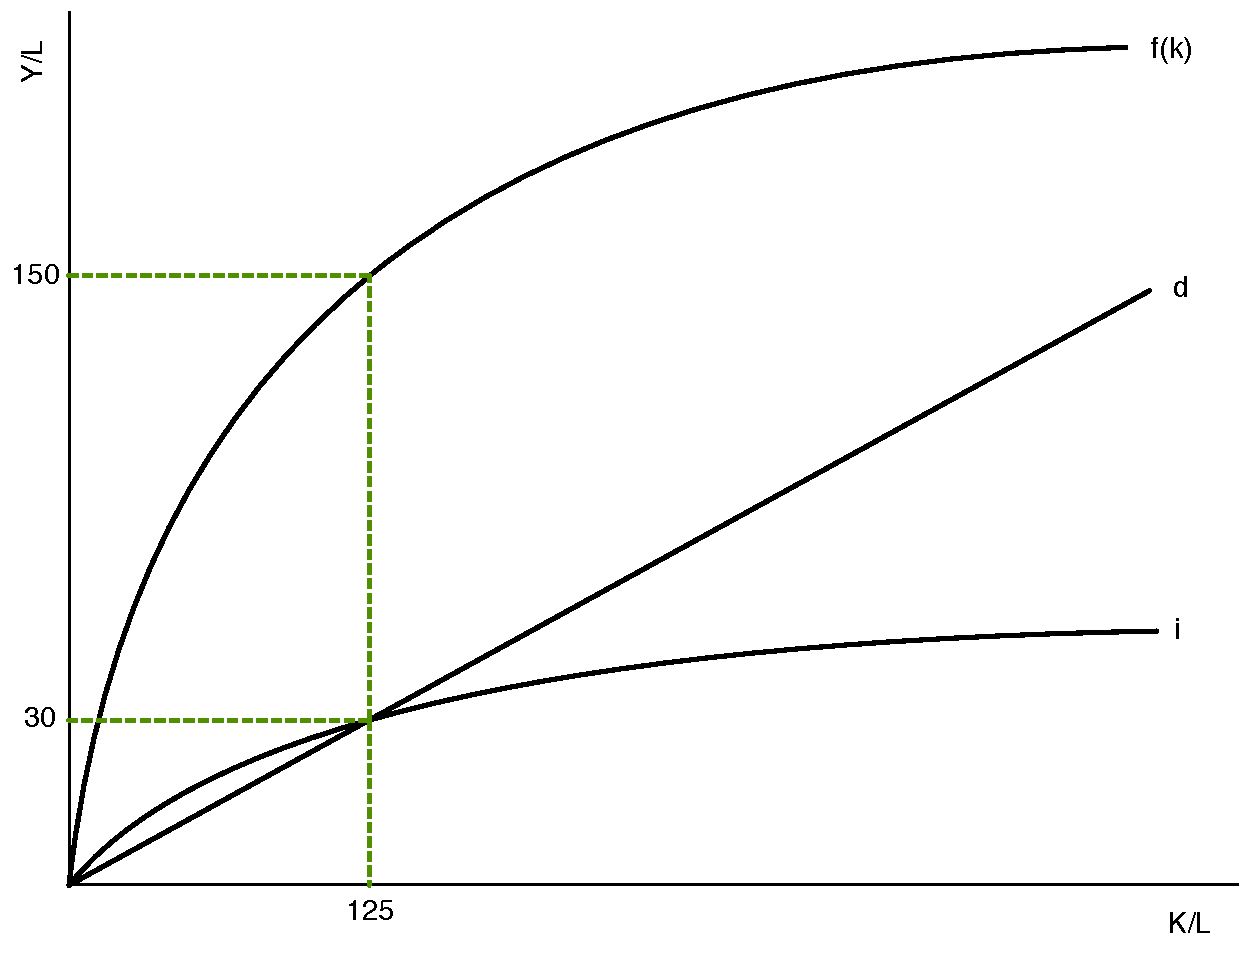
\includegraphics[scale=.35]{Final_MC22.pdf}
		\caption{Production, Investment, and Depreciation}
		\label{MC22}
	\end{figure}
	
	The percent of output per worker that is invested every period is \blank and the rate of capital depreciation is \blank.
	
	\begin{choices}
		\choice 20\%; 20\%
		\choice 24\%; 20\%
		\choice 24\%; 24\%
		\CorrectChoice 20\%; 24\%
	\end{choices}
	
\newpage
	
	\question Institutions are thought to be the \blank causes of economic growth.
	
	\begin{choices}
		\choice proximate
		\choice immediate 
		\CorrectChoice ultimate
		\choice direct
	\end{choices}
	
	\question Which of the following is NOT considered an investment for calculating GDP?
	
	\begin{choices}
		\choice A family purchases a new home.
		\CorrectChoice An investor purchases Apple stock.
		\choice A farmer buys a new tractor.
		\choice KIA Motors builds a new factory.
	\end{choices}
	
	\question A country experiencing low GDP growth and high population growth will have a
	
	\begin{choices}
		\choice low real GDP growth rate.
		\choice low nominal GDP growth rate.
		\CorrectChoice low per capita GDP growth rate.
		\choice high per capita GDP growth rate.
	\end{choices}
	
	\question This weekend, your friends invite you to see a concert in Charlotte. Tickets are \$15 each, but your friends know you are financially constrained and offer to buy you the ticket as long as you chip in \$10 for gas. On the other hand, you could go for a relaxing hike. The park you go to charges \$1 for parking, and generally you would be willing to pay \$5 for the opportunity to enjoy Mother Nature. Based on this information, what is the opportunity cost of going to the concert with your friends?
	
	\begin{choices}
		\CorrectChoice \$14
		\choice \$10
		\choice \$16
		\choice \$15
	\end{choices}
	
	\question A firm is producing 500 units with an average total cost of \$10 and a marginal cost of \$15. If it were to increase production to 501 units, which of the following must occur?
	
	\begin{choices}
		\choice Marginal cost would decrease.
		\choice Marginal cost would increase.
		\choice Average total cost would decrease.
		\CorrectChoice Average total cost would increase.
	\end{choices}


	\question The cost of a basket of goods and services in 1990 was computed to be \$90. In 2000, this same basket's cost was computed to be \$85. Moreover, the CPI in 2001 using 1990 as the base year was 90. What was the inflation rate between 2000 and 2001?
	
	\begin{choices}
		\choice $-5.88\%$
		\choice 4.70\%
		\CorrectChoice $-4.70\%$ 
		\choice 5.88\%
	\end{choices}
	
	\question Suppose that changes in the market for ice cream caused the equilibrium price to increase and the equilibrium quantity to decrease today. Which of the following \textit{could} have caused this outcome?
	
	\begin{choices}
		\CorrectChoice Buyers and sellers hear that Ben and Jerry's, a major seller of ice cream, will go out of business in six months time.
		\choice The First Lady begins a public awareness campaign about the benefits of eating a cup of ice cream a day.
		\choice The government imposes a maximum price that sellers can charge for each quart of ice cream.
		\choice The government does away with the minimum wage, causing wages paid to workers in ice cream factories to decrease.
		\choice Either (a) or (c)
	\end{choices}
	

	
	\question Which of the following examples demonstrates the free rider problem?
	
	\begin{choices}
		\CorrectChoice Josh downloads the podcast \textit{Serial}, but never contributes to NPR, its producer.
		\choice Liz Lemon is upset that she and Jack Donaghy pay the same amount at the toll booth, even though she only uses the road for 5 miles, while he uses it for 25 miles.
		\choice Due to a lack of clearly defined property rights, ocean creatures tend to be overfished.
		\choice Kristina, Jane, and Andrea rent three movies and enforce that the costs are split evenly, even though Jane is only willing to pay her share for two movies.
	\end{choices}
	
	\question As individuals lose their jobs, they buy more potatoes. Which of the following might be the income elasticity of demand for potatoes?
	
	\begin{choices}
		\choice $-1.32$
		\choice $.54$
		\choice $-.30$
		\CorrectChoice Either (a) or (c)
	\end{choices}
	
	\question Which of the following is NOT a determinant of a country's long-run productivity?
	
	\begin{choices}
		\choice Natural resources
		\choice Human capital
		\CorrectChoice Money supply
		\choice Physical capital
	\end{choices}
	
	
	\question John Doe looked for a new job for two months when he and his family moved to South Florida, but stopped looking for work six weeks ago because his wife landed a prominent position at the University of Miami. As of right now, John is considered \blank by the BLS.
	
	\begin{choices}
		\choice frictionally unemployed
		\choice structurally unemployed 
		\choice cyclically unemployed
		\CorrectChoice not in the labor force
	\end{choices}
	
	
	\question Consider Figure \ref{MC33}, which shows the impact of a negative real shock.
	
	
	\begin{figure}[H]
		\centering
		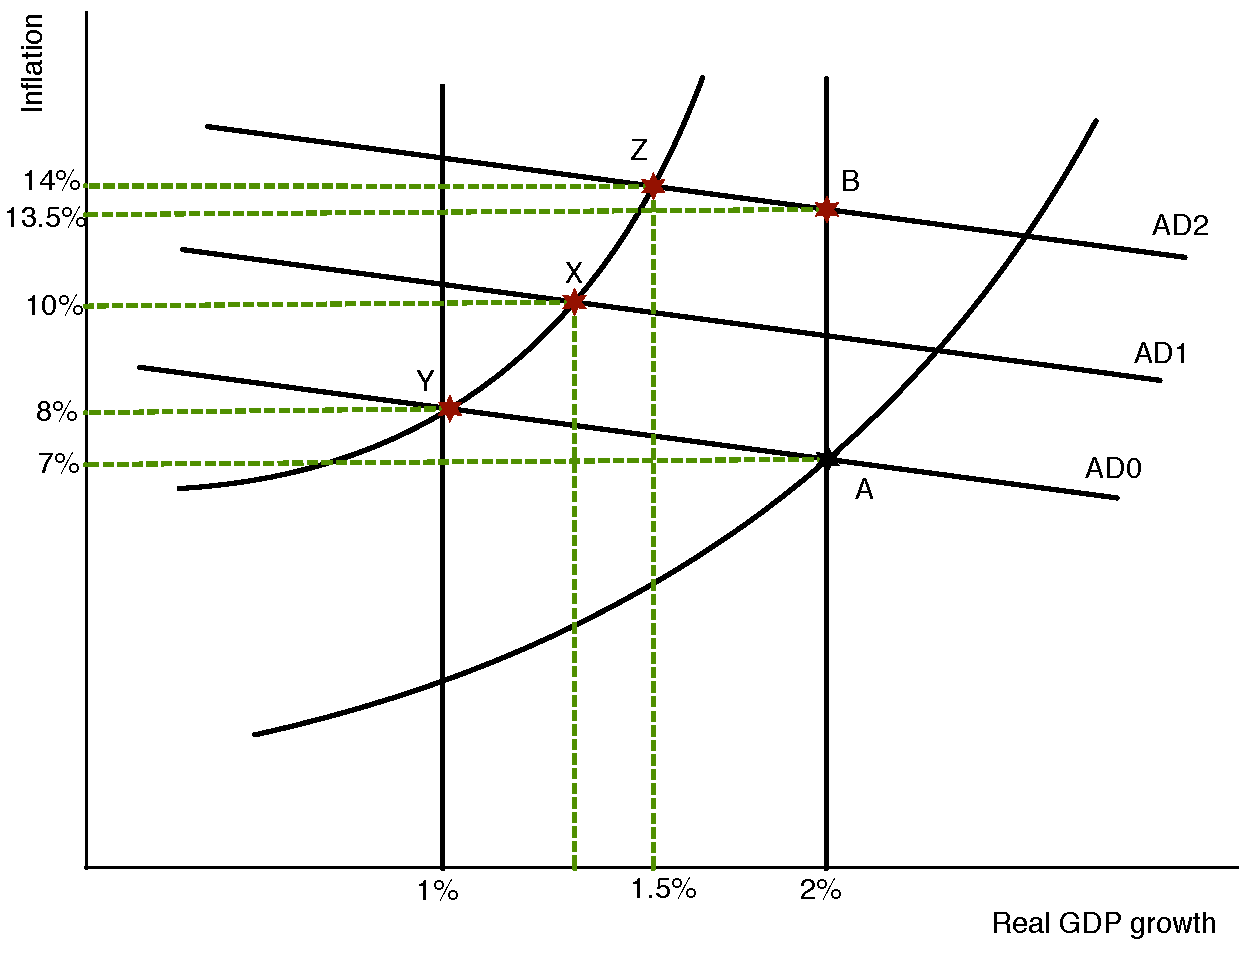
\includegraphics[scale=.38]{ec2_plot1.pdf}
		\caption{Real Shock}
		\label{MC33}
	\end{figure}
	
	Assume that after the shock, the economy is operating at point $Y$. Now, suppose fiscal policy is enacted that shifts aggregate demand to AD1, and this spurs consumer spending so that aggregate demand shifts further to AD2. In the absence of crowding out, the economy will experience real GDP growth of \blank and an inflation rate of \blank in the short run.
	
	\begin{choices}
		\CorrectChoice 1.5\%; 14\%
		\choice 2\%; 7\%
		\choice 2\%; 13.5\%
		\choice 1.4\%; 10\%
	\end{choices}
	
	\question Suppose an economy contains 2,000 \$1 bills. If people initially deposit half their currency as demand deposits while banks maintain 100\% reserves, the quantity of money would be \blank. If, however, people initially deposit all their currency as demand deposits while banks maintain 100\% reserves, the quantity of money is \blank.
	
	\begin{choices}
		\choice \$2,000; \$1,000
		\choice \$1,000; \$1,000
		\choice \$1,000; \$2,000
		\CorrectChoice \$2,000; \$2,000
	\end{choices}
	
	\question Consultants hired by Sunnyside Eggs find that the firm has average fixed costs of \$40, average variable costs of \$35, and an average revenue of \$40. Given this, in the short run the firm should \blank and make \blank profit.
	
	\begin{choices}
		\choice shut down; negative
		\choice shut down; zero
		\CorrectChoice stay open; negative
		\choice stay open; positive
	\end{choices}
	
	\question Consider Figure \ref{MC35}, which shows the cost structure of a monopolist.
	
	\begin{figure}[H]
		\centering
		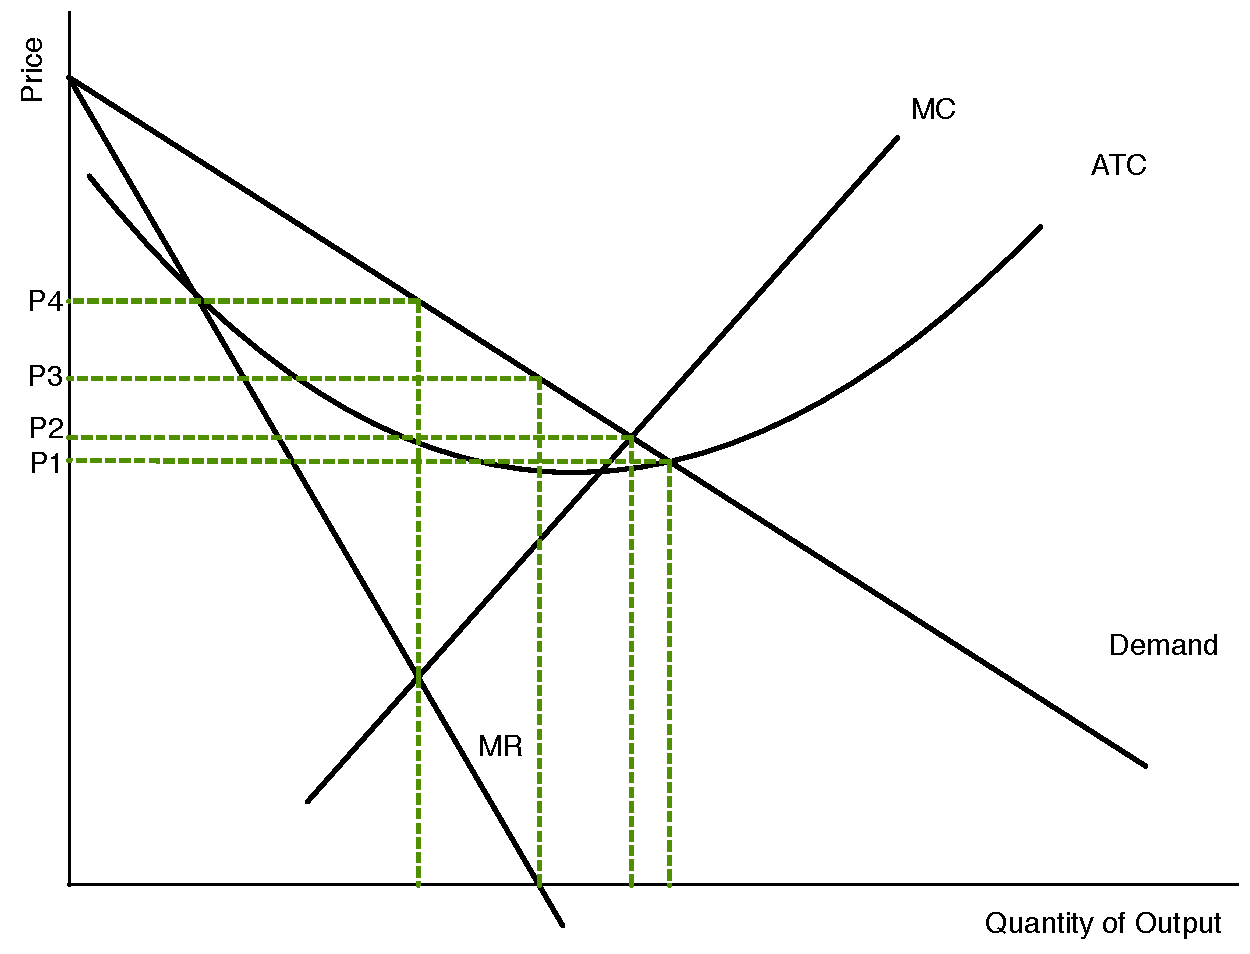
\includegraphics[scale=.40]{Final_MC35.pdf}
		\caption{Monopolist Environment}
		\label{MC35}
	\end{figure}
	
	If the firm wishes to maximize total revenue, it should charge price \blank, while the price it should charge to maximize output while not making losses is \blank.
	
	\begin{choices}
		\choice P4; P2
		\CorrectChoice P3; P1
		\choice P2; P4
		\choice P3; P2
		\choice None of the above
	\end{choices}
	

	
	\question Suppose that a permanent decrease in investment spending causes a recession. If the Fed wishes to counteract this change in aggregate demand in order to get the economy back to its initial real GDP growth rate, it could
	
	\begin{choices}
		\choice sell bonds.
		\choice increase the interest rate on reserves.
		\CorrectChoice lower the discount rate. 
		\choice increase reserve requirements.
		\choice None of the above achieves this goal.
	\end{choices}
	
	
	\question Suppose the market for corn is perfectly competitive. Which of the following represents the long-run relationship between the price, marginal cost, and average total cost at the profit-maximizing quantity?
	
	\begin{choices}
		\choice $P > MC = ATC$
		\choice $P = MC > ATC$ 
		\CorrectChoice $P = MC = ATC$
		\choice $P > MC > ATC$
	\end{choices}
	
\newpage
	
	\question In order to eliminate the deadweight losses associated with a negative market externality, the government should impose a per unit tax \blank.
	
	\begin{choices}
		\choice equal to the total external cost
		\choice less than the total external cost
		\choice greater than the per unit external cost.
		\CorrectChoice equal to the per unit external cost.
		\choice None of the above.
	\end{choices}
	
	\question Suppose a shift in the money supply caused the value of money to decrease from $1/4$ to $1/5$. As such, the price level in the economy
	
	\begin{choices}
		\choice decreased 20\%.
		\CorrectChoice increased 25\%.
		\choice increased 20\%.
		\choice decreased 25\%.
	\end{choices}
	
	\question Refer to Table 1, which gives the willingness to pay for 1 lb of kale of four individuals.
	
	\begin{table}[H]
		\caption{WTP for 1 lb Kale}
		\centering
		\begin{tabular}{ c| c}        
			
			\hspace{1cm} Buyer \hspace{1cm}   & \hspace{1cm} WTP \hspace{1cm} \\
			\hline
			Natalie & \$4.00 \\
			Avery & \$1.00 \\
			Meredith & \$3.50 \\
			Madi & \$.50 \\
		\end{tabular}
		
	\end{table} 
	
	If the market price for kale is \$1.00, the total consumer surplus realized is
	
	\begin{choices}
		\choice \$5.00
		\CorrectChoice \$5.50
		\choice \$4.00
		\choice \$3.00
	\end{choices}
	
	\question If the government wishes to impose a \$5 per unit tax on sellers, but wishes to minimize the deadweight losses resulting from the tax, it should impose the tax on a market 
	
	\begin{choices}
		\choice with elastic demand and inelastic supply.
		\choice with inelastic demand and elastic supply.
		\CorrectChoice with inelastic demand and inelastic supply.
		\choice with elastic demand and elastic supply.
	\end{choices}

	\question When workers lose their jobs and become officially unemployed, the labor force participation rate
	
	\begin{choices}
		\choice increases. 
		\CorrectChoice remains constant.
		\choice decreases.
		\choice Any of the above could occur.
	\end{choices}
	
	
	\question Suppose a price ceiling of \$300 is imposed in the market shown in Figure \ref{MC42}.
	
	
	\begin{figure}[H]
		\centering
		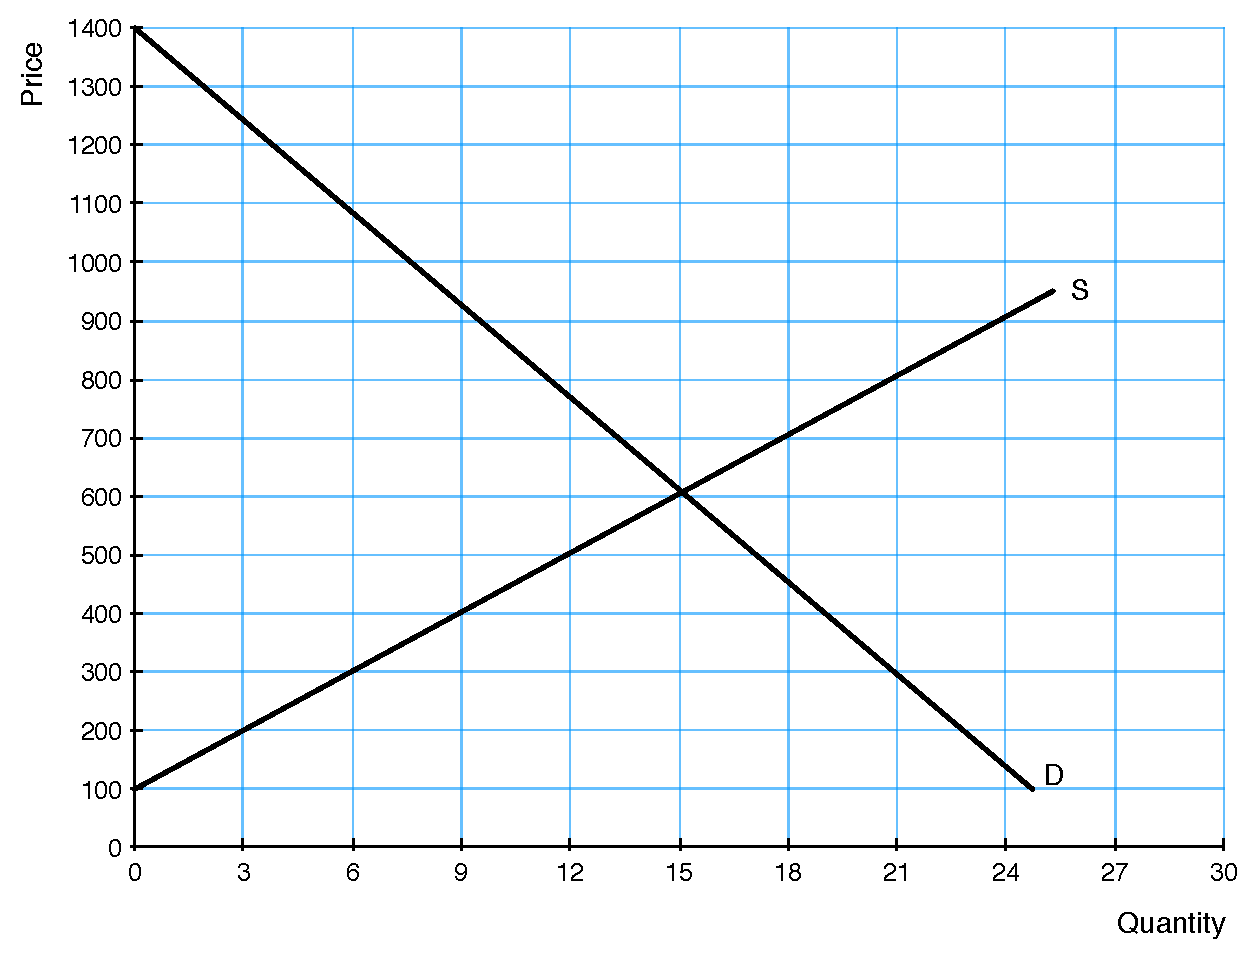
\includegraphics[scale=.40]{Final_MC42.pdf}
		\caption{Market for Surface Tablets}
		\label{MC42}
	\end{figure}
	
	As a result, there is a \underline{\hspace{3cm}} and deadweight losses of \underline{\hspace{3cm}}.
	
	\begin{choices}
		\choice shortage of 15 units; \$7,200
		\choice surplus of 6 units; \$7,200
		\choice shortage of 6 units; \$3,600
		\choice surplus of 15 units; \$3,600
		\CorrectChoice None of the above.
	\end{choices}
	


	
	\question What effect will an investment tax credit have on interest rates and the quantity of savings?
	
	\begin{choices}
		\choice both interest rates and the quantity of savings will decrease.
		\choice interest rates will increase, and the quantity of savings will decrease.
		\CorrectChoice both interest rates and the quantity of saving will increase. 
		\choice interest rates will decrease, and the quantity of savings will increase.
	\end{choices}
	

	\question Which of the following is NOT a tool the Fed uses to influence the money supply?
	
	\begin{choices}
		\CorrectChoice Raise/lower taxes
		\choice Purchase/sell bonds
		\choice Pay interest on reserves
		\choice Set reserve requirements
		\choice None of the above
	\end{choices}	
	
	\question An AM transmission of a baseball game is a \blank because it is \blank.
	
	\begin{choices}
		\choice private good; rival and excludable
		\choice club good; rival and non-excludable
		\CorrectChoice public good; non-rival and non-excludable
		\choice common resource; non-rival and excludable
	\end{choices}
	
	\question Suppose a country is currently at its steady state. If the country's population growth rate permanently increases from 2\% to 4\%, which of the following must be true?
	
	
	\begin{enumerate}[i.]
		\item Consumption will immediately increase, and the new steady state consumption level will be greater than the old steady state consumption level.
		\item Investment will immediately decrease, and the new steady state investment level will be less than the old steady state investment level.
		\item The new steady state level of capital will be less than the old steady state level of capital, and the new steady state level of output will be less than the old steady state level of output.
	\end{enumerate}
	
	\begin{choices}
		\choice i and ii
		\choice ii and iii
		\choice i only
		\CorrectChoice iii only
		\choice i, ii, and iii
	\end{choices}
	

	
	\question Unexpected deflation will
	
	\begin{choices}
		\choice lower the real value of debts and redistribute wealth from lenders to borrowers.
		\choice lower the real value of debts and redistribute wealth from borrowers to lenders.
		\choice raise the real value of debts and redistribute wealth from lenders to borrowers.
		\CorrectChoice raise the real value of debts and redistribute wealth from borrowers to lenders.
	\end{choices}
	

	
	\item Stella's Bakery makes fresh bread every morning at 6:00AM and throws out any remaining bread at closing time, 4:00PM. They sell the bread for \$3.50 a loaf and it costs them \$1.25 to make each one. Every customer at Stella's pay with a credit card and only buys one loaf of bread. Additionally, Stella's is charged \$.25 by the credit card company for each transaction that takes place. The manager has 30 loafs of bread left over at 3:30PM today. Assuming throwing the bread away is costless, which of the following alternatives is most attractive?
	
	\begin{choices}
		\choice Lower the price of the remaining bread, but no lower than \$1.25.
		\CorrectChoice Lower the price of the remaining bread, but no lower than \$.25.
		\choice Lower the price of the remaining bread, but no lower than \$1.00.
		\choice Lower the price of the remaining bread, even if it falls below \$.25.
	\end{choices}


\end{questions}

\newpage

\section*{Short Answer}

For this section, make sure to write legibly and box final answers. \textbf{Show your work!} This can be done within the section or \textit{clearly} labeled on the scratch paper provided.

\begin{questions}
	
	\question Suppose that an economy has a natural growth rate of 2\%. Moreover, the central bank in the country has perfect control over the money supply and increases it by 4\% every year. Assume spending is such that the velocity of money is constant over time and that the economy is currently at its long-run equilibrium.
	
	\begin{parts}
		
		\part[2] Draw a clearly labeled dynamic AS-AD diagram that shows the long-run equilibrium point, as well as the economy's current growth rate of real GDP, inflation, and expected inflation. Label this point $E_0$. Be sure to include both the short-run and long-run aggregate supply curves. 
		\vspace{4cm}
		
		\part[2] Now, suppose that the stock market declines sharply, reducing consumers' wealth. As a result, consumers spend at a rate that is 4\% lower than before. Assume this change is permanent. Does this affect aggregate demand, short-run aggregate supply, or long-run aggregate supply? Explain why. 
		\vspace{2cm}
		
		\part[3] Show this change graphically in part (a). Assume that neither the central bank nor the federal government enact any policies to counteract this change. Label the short-run equilibrium point $A$ and the long-run equilibrium point $E_1$. What is the inflation rate in the short run if this change in consumer spending caused real GDP growth to decrease to $-1\%$? What will be the long-run real GDP growth rate and inflation rate? 
		\vspace{1cm}
		
		\part[3] Explain why the short-run growth rate of output is different from the long-run growth rate of output. What causes the economy to move from point $A$ to point $E_1$? 
		\vspace{1.5cm}
		
		\part[2] Now, suppose the central bank decides to intervene while the economy is at point $A$. State two policies \textit{the central bank} could enact to get the economy back to point $E_0$. Be specific as to which curve is affected. 
		\vspace{1cm}
		
		\part[3] Regardless of the policy pursued, show how this policy would be reflected graphically in part (a). Specify what the growth rate of the money supply must be in order for this policy to achieve its goal. 
		\vspace{1cm}
		
	\end{parts}

	
	\question Suppose nominal GDP in an economy is \$5,000, real GDP is \$1,250, and the money supply is \$2,500. 
	
	\begin{parts}
		\part[3] What is the price level in the economy, the value of money in the economy, and the velocity of money? 
		\vspace{1cm}
		
		\part[3] Suppose that velocity is constant and the economy's output of goods and services increases 3\% over the course of the year. If the Fed increases the money supply in the economy 4\% every year, what happens to the growth rate of nominal GDP and the price level?
		 \vspace{1cm}
		 
		\part[2] What should the \textit{level} of the money supply be next year if the Fed wishes to have inflation of 5\%? 
		\vspace{1cm}
		
		\part[2] It is sometimes suggested that the Fed should try to target zero inflation. If we assume constant velocity, does this zero-inflation goal require that the rate of money growth be zero? If yes, explain why. If no, explain what the rate of money growth should equal both in general AND in the context of this problem. 
		\vspace{1cm}
		
	\end{parts}
	
\end{questions}
		

\hrulefill
\begin{center} 
	\textbf{END OF EXAM}
\end{center}

\newpage

\centering

\section*{SCRATCH SHEET}


\end{document}